%--------------------------------------------------------------------
%--------------------------------------------------------------------
% Formato para los talleres del curso de Métodos Computacionales
% Universidad de los Andes
% 2015, curso de vacaciones
%--------------------------------------------------------------------
%--------------------------------------------------------------------

\documentclass[11pt,letterpaper]{exam}
\usepackage[utf8]{inputenc}
\usepackage[spanish]{babel}
\usepackage{graphicx}
\usepackage{mdframed}
\usepackage{tabularx}
\usepackage[absolute]{textpos} % Para poner una imagen en posiciones arbitrarias
\usepackage{multirow}
\mdfdefinestyle{mystyle}{leftmargin=1cm,rightmargin=1cm,linecolor=red}
\usepackage{float}
\usepackage{hyperref}
\decimalpoint

\newcommand{\base}[1]{\underline{\hspace{#1}}}
\boxedpoints
\pointname{ pt}
%\extrawidth{0.75in}
%\extrafootheight{-0.5in}
\extraheadheight{-0.15in}
\hypersetup{%
  colorlinks=true,% hyperlinks will be coloured
  urlcolor=blue
}

%\noprintanswers
%\printanswers
\renewcommand{\solutiontitle}{}
\SolutionEmphasis{\color{blue}}

\usepackage{upquote,textcomp}
\newcommand\upquote[1]{\textquotesingle#1\textquotesingle} % To fix straight quotes in verbatim
\newcommand{\ihat}{\,\hat{\textbf{\i}}}
\newcommand{\jhat}{\,\hat{\textbf{\j}}}

\begin{document}
\begin{center}
{\Large Métodos Computacionales} \\
Tarea 5 - \textsc{ODE} \\
Julio de 2015
\end{center}

\begin{textblock*}{40mm}(10mm,20mm)
  
\includegraphics[width=3cm]{logoUniandes.png}
\end{textblock*}

\begin{textblock*}{40mm}(164mm,20mm)
  
\includegraphics[width=3cm]{logoUniandes.png}
\end{textblock*}

\vspace{0.5cm}

La solución a esta tarea debe cargarse a su repositorio en GitHub en la carpeta /MC/Tareas/HW5/ y debe contener el cuaderno \verb+HW5.ipynb+ y los archivos de las dos animaciones. En el cuaderno dedicar una sección a cada ejercicio con subsecciones para cada literal. Es requisito que en todo lo hecho se pongan comentarios que expliquen lo que se está haciendo.  

La fecha límite de entrega es el \textbf{jueves 2 de julio a las 23:59}. Puede trabajarse en parejas.

%\begin{textblock*}{100mm}(-430mm,130mm)
%  
\includegraphics[width=80cm]{koch6_tight.pdf}
%\end{textblock*}

\begin{textblock*}{100mm}(-9mm,-17mm)
  
\includegraphics[width=22cm]{tangle2.pdf}
\end{textblock*}

\vspace{0.5cm}

\begin{questions}
 
\question[50] \textbf{3-Coreografía} \\
\begin{parts}
\part[20] Resuelva las ecuaciones de movimiento para tres cuerpos de igual masa sujetos a su mutua atracción gravitacional con las siguientes condiciones iniciales:

\[ \vec{r}_1\left(0\right) =  a \ihat  + b \jhat, \quad \vec{v}_1\left(0\right) = c \ihat + d \jhat, \]
\[ \vec{r}_2\left(0\right) =  -a \ihat  - b \jhat, \quad \vec{v}_2\left(0\right) = c \ihat + d \jhat, \]\\[-0.8cm]
\[ \vec{r}_3\left(0\right) =  0 \ihat  + 0 \jhat, \quad \vec{v}_3\left(0\right) = -2(c \ihat + d \jhat), \]
\[ \textrm{donde} \]
\[ a =  0.24250109\quad b=-0.0607718825\]
\[ c = 0.93240737 \quad d = 0.86473146.\]

Tome $G=1$ y use el método de Runge-Kutta de orden 4. Integre las ecuaciones de movimiento para media unidad de tiempo.

\begin{center}
	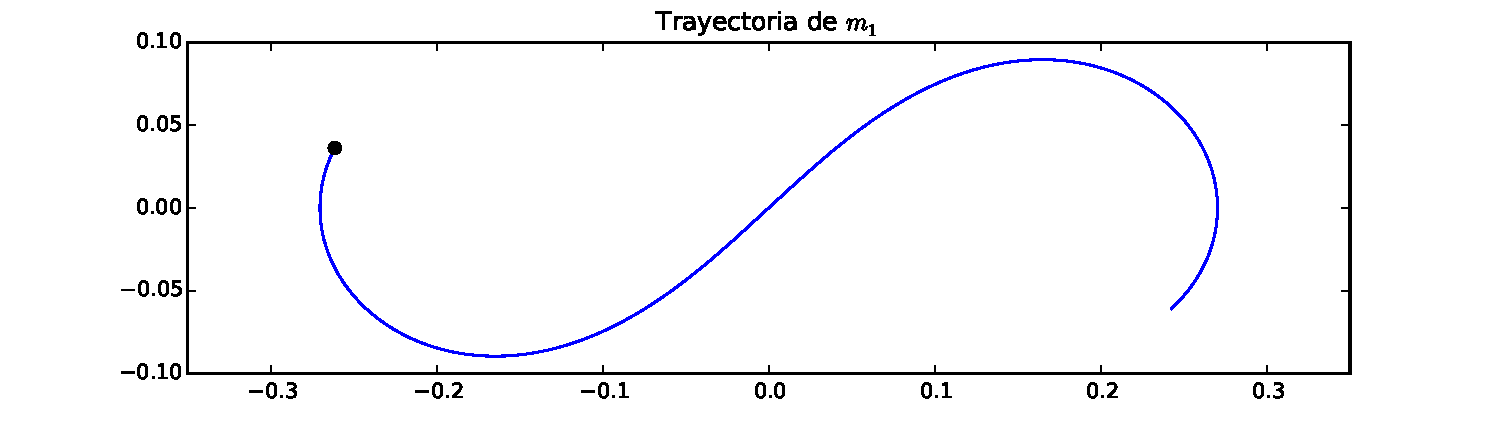
\includegraphics[width=0.95\textwidth]{./halfunit.pdf}
\end{center}

\part[20] Las trayectorias son periódicas, calcule el periodo con por lo menos tres cifras significativas.

\part[10] Haga una animación similar a \href{https://github.com/ComputoCienciasUniandes/MetodosComputacionales/raw/master/homework/2015-V/HW5/grav_choir.mp4}{esta}.

\end{parts}

%\vfill
%\begin{center}
%
\includegraphics[width=0.9\textwidth]{tangle.pdf}
%\end{center}
%\vfill
\newpage

\question[50] \textbf{4-Coreografía} \\

Cuatro masas bajo la influencia de su mutua fuerza de gravedad y siguientes condiciones iniciales tienen un movimiento periódico para cierto valor de $a$. $(m_1=m_2=m_3=m_4=G=1)$


\[\vec{r}_1\left(0\right)=0.384277200514 \ihat + 0.0 \jhat\]
\[\vec{r}_2\left(0\right)=-0.0156823005697 \ihat -0.13966430504 \jhat\]
\[\vec{r}_3\left(0\right)=-0.352912599375 \ihat + 0.0 \jhat\]
\[\vec{r}_4\left(0\right)=-0.0156823005697 \ihat + 0.13966430504 \jhat\]
\[\quad\quad\quad\quad\quad\quad\quad\quad\quad\quad\quad\quad\quad\quad\quad\quad\quad\quad\vec{v}_1\left(0\right)=0.0 \ihat + a \jhat \leftarrow \textrm{INCÓGNITA}\]
\[\vec{v}_2\left(0\right)=-2.01155925929 \ihat -1.19817066623 \jhat\]
\[\vec{v}_3\left(0\right)=0.0 \ihat + 1.63619158614 \jhat\]
\[\vec{v}_4\left(0\right)=2.01155925929 \ihat -1.19817066623 \jhat\]
\[ \textrm{donde} \]
\[0.70 < a < 0.78.\]

\begin{parts}
\part[30] Encuentre $a$ con cinco cifras significativas. Piense en una función objetivo que tenga un mínimo en la condición deseada, y cuando halla reducido el intervalo de búsqueda lo suficiente piense en otra que cambie de signo en la condición deseada.

\begin{center}
	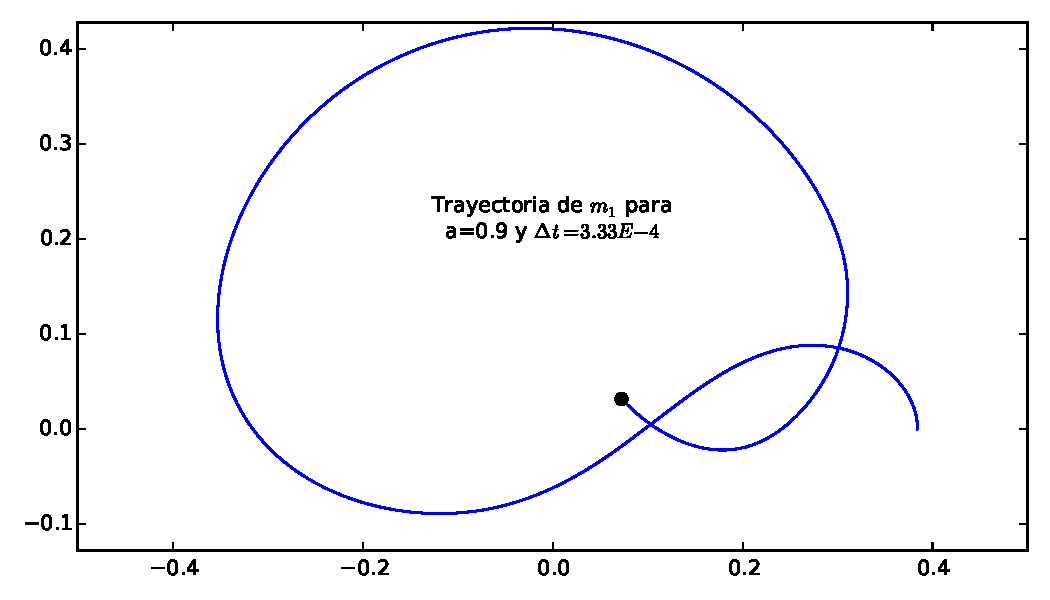
\includegraphics[width=0.95\textwidth]{ex_trayectory.pdf}
\end{center}
\newpage
\part[10] Con el valor de $a$ encontrado haga una gráfica con la energía cinética, la energía potencial y la energía total del sistema en función del tiempo.

\begin{center}
	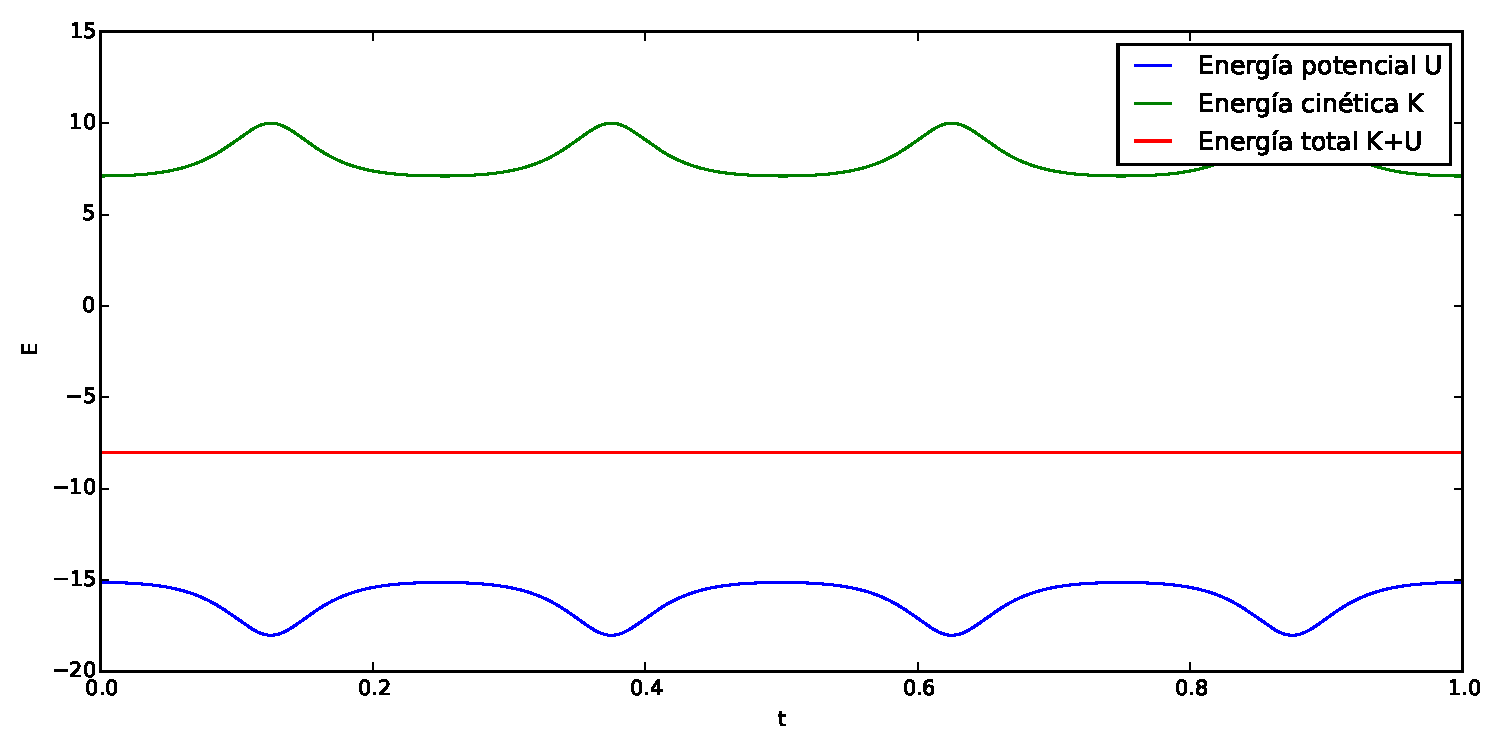
\includegraphics[width=0.95\textwidth]{energyplot.pdf}
\end{center}

\part[10] Haga una animación de las trayectorias de los cuatro cuerpos.
\end{parts}
\end{questions}



\end{document}
